\chapter{Motion Law}%
\label{chap:motion_law}

	The path found with the algorithms described in
	Chapter~\ref{chap:path_processing} can be considered as a continuous smooth
	mapping that adheres to:

	\begin{equation}
		\pathsym : \timenorm \in [0, 1] \mapsto \specialEuclideanGroup{3}
			\quad
			\suchthat
			\quad
			\pathsym(0) = \pose_{\initial}, \pathsym(1) = \pose_{\goal}
	\end{equation}

	If $\timenorm$ is interpreted as time, then it would imply that the robot is
	in its initial pose at $\timesym = 0\si{\second}$ and reaches its goal pose
	at $\timesym = 1\si{\second}$. While $\pathsym$ is guaranteed to be free of
	collisions, this interpretation makes no guarantee that the actuators can
	move the end-effector this fast. For this reason, a motion law,
	$\motionlaw$, must be found that performs the following mapping:

	\begin{equation}
		\motionlaw: \timesym\in\Re \mapsto \timenorm\in[0, 1]
	\end{equation}

	The trajectory, $\traj:\timesym \mapsto \specialEuclideanGroup{3}$, can then
	be defined simply as:

	\begin{equation}
		\traj = \pathsym(\motionlaw(\timesym))
	\end{equation}

	In addition to the no-collision guarantees of $\pathsym$, $\traj$ also
	guarantees that the actuators stay within their saturation ranges. The
	present chapter describes the approach followed to find a suitable
	$\motionlaw$.

	\section{Motion Law Generation Algorithm}%
\label{sec:motion_law_generation_algorithm}

	Since the actuators work directly on the length of the cables, the
	search for a suitable motion law $\motionlaw$ is performed in cable
	space and not in pose space. As a first step, $\timenorm$ is considered
	to be linked directly to time, $\timesym \defeq \timenorm$, and the
	cable velocities along the resulting trajectory is then found as:

	\begin{equation}
		\dot{\cablevec}(\timenorm) =
			\invgeometricmodel
			\left(
				\frac
				{%
					\der\pathsym
				}
				{%
					\der\timesym
				}
			\right)
	\end{equation}

	Each cable in $\cablevec$ is subjected to kinematic constraints on its
	velocity, $\dot\cablelength_{\max}$\todo{also discuss acceleration, jerk
	etc when implemented}.  That is, each cable has a maximum velocity which
	it may not exceed. As such, the next step in the algorithm is finding
	the ranges that exceed this maximum velocity. In other words, find the
	set of time instants $\timenorm$ where:

	\begin{equation}
		\abs{\dot{\cablevec}(\timenorm)} \geq \dot{\cablevec}_{\max}
		\label{eq:excessive_cable_velocity}
	\end{equation}

	In general, there may be multiple ranges along the trajectory where the
	maximum velocity in Equation~\ref{eq:excessive_cable_velocity} is
	exceeded. A range in $\timenorm$, $\rangetimenorm$, is encapsulated as
	the ordered tuple:

	%\begin{equation}
	%	\rangetimenorm =
	%		\left(
	%			\timenorm_{\min},
	%			\timenorm_{\max}
	%		\right)
	%	%
	%\end{equation}

	%such that

	%\begin{equation}
	%	\abs
	%	{%
	%		\dot{\cablevec}
	%			(
	%				\timenorm
	%			)
	%	}
	%	%
	%	\geq \dot{\cablevec}_{\max}
	%	\quad
	%	\forall\timenorm\in[\timenorm_{\min}, \timenorm_{\max}]
	%\end{equation}

	%and

	%\begin{align}
	%	\begin{split}
	%		\dot{\cablevec}(\timenorm_{\min}^-) &< \dot{\cablevec}_{\max} \\
	%		\dot{\cablevec}(\timenorm_{\min}^+) &> \dot{\cablevec}_{\max} \\
	%		\dot{\cablevec}(\timenorm_{\max}^-) &> \dot{\cablevec}_{\max} \\
	%		\dot{\cablevec}(\timenorm_{\max}^+) &< \dot{\cablevec}_{\max} \\
	%	\end{split}
	%\end{align}

	\begin{equation}
		\rangetimenorm =
			\left(
				\timenorm_{\min},
				\timenorm_{\max}
			\right)
		%
		\quad
		\suchthat
		\quad
		%
		\begin{cases}
			\abs
			{%
				\dot{\cablevec}
					(
						\timenorm
					)
			}
			\geq \dot{\cablevec}_{\max}
			\forall\timenorm\in[\timenorm_{\min}, \timenorm_{\max}]\\
			%
			\dot{\cablevec}(\timenorm_{\min}^-) < \dot{\cablevec}_{\max} \\
			\dot{\cablevec}(\timenorm_{\min}^+) > \dot{\cablevec}_{\max} \\
			\dot{\cablevec}(\timenorm_{\max}^-) > \dot{\cablevec}_{\max} \\
			\dot{\cablevec}(\timenorm_{\max}^+) < \dot{\cablevec}_{\max} \\
		\end{cases}
	\end{equation}

	Note that the following notation is used to test whether a value is in a
	range:

	\begin{equation}
		\timenorm \in \rangetimenorm =
			\begin{cases}
				\true, \quad \timenorm \in [\timenorm_{\min},
				\timenorm_{\max}] \\
				\false, \quad\text{otherwise}
			\end{cases}
	\end{equation}

	All such ranges are put into an ordered set of ranges,
	$\setofrangestimenorm$, such that:

	\begin{equation}
		{\rangetimenorm}_{\indexi} \prec
		{\rangetimenorm}_{\indexj} \iff
		{\rangetimenorm}_{\indexi}\code{.}{\timenorm_{\max}} <
		{\rangetimenorm}_{\indexj}\code{.}{\timenorm_{\min}}
	\end{equation}

	$\setofrangestimenorm$ is then used as an input to the algorithms that
	generate $\motionlaw$.

	The idea behind the algorithm is now to simply scale the time in such a
	way that:

	\begin{equation}
		\frac
		{%
			\der\timesym
		}
		{%
			\der\timenorm
		}
		=
		\begin{cases}
			1, \quad \timenorm \notin \setofrangestimenorm \\
			\gain_{\indexi}, \quad \timenorm \in {\rangetimenorm}_{\indexi}
		\end{cases}
		\forall{\rangetimenorm}_{\indexi}\in\setofrangestimenorm
	\end{equation}

	Where $\gain_{\indexi}$ is chosen such that, for the currently active
	${\rangetimenorm}_{\indexi}$:

	\begin{equation}
		\abs
		{%
			\dot{\cablevec}(\timenorm)
		}
		\leq \dot{\cablevec}_{\max}
		\quad\forall{\timenorm}\in{\rangetimenorm}_{\indexi}
	\end{equation}
	\todo{describe how $\gain_{\indexi}$ is chosen}

	A graphical intuition of the algorithm is given in
	Figure~\ref{fig:motion_law_graphical_intuition}. The top graph shows the
	velocity profile of a single cable for a given path
	$\pathsym(\timenorm)$. It also highlights the set $\setofrangestimenorm$
	that exceed the maximum velocities. The middle graph shows schematically
	how the motion law $\motionlaw:\timesym \mapsto \timenorm$ is
	generated. Finally, the bottom graph shows the effect of applying
	$\motionlaw$ to $\pathsym$ to obtain a trajectory $\traj(\timesym)$
	which no longer exceeds maximum velocities.

	\begin{figure}[hb]
		\centering
		\def\svgheight{8cm}
		\import{res/img/}{motion_law_intuition.pdf_tex}
		\caption{Motion Law Construction}%
		\label{fig:motion_law_graphical_intuition}
	\end{figure}

	\todo{put algorithm here}

	The motion law shown in Figure~\ref{fig:motion_law_graphical_intuition}
	will guarantee that the velocity constraints of the actuators are
	respected. However, the corners in this graph correspond to sudden
	changes in the rate at which $\pathsym$ is followed and can lead to
	excessive accelerations in the cables. For this reason, instead of using
	the motion law as it is presented in
	Figure~\ref{fig:motion_law_graphical_intuition}, the corners are used as
	control points which can then be interpolated using a B-spline of
	sufficient degree. A B-spline of degree two can guarantee continuous
	accelerations. Higher-degree B-splines guarantee continuity in higher
	time derivatives of $\traj$.


	\section{Sample Motion Law Processing Output}%
\label{sec:sample_motion_law_processing_output}

	The current section shows and discusses sample output of the algorithm
	described in Section~\ref{sec:motion_law_generation_algorithm}. The current
	discussion relates to the planning problem and trajectory of
	Figure~\ref{fig:motion_law_sample_problem}.

	\begin{figure}[hb]
		\begin{minipage}{0.5\textwidth}
			\centering
			\includegraphics[height=0.6\textwidth]{kinematic_scaling_base_problem}
		\end{minipage}
		\begin{minipage}{0.5\textwidth}
			\centering
			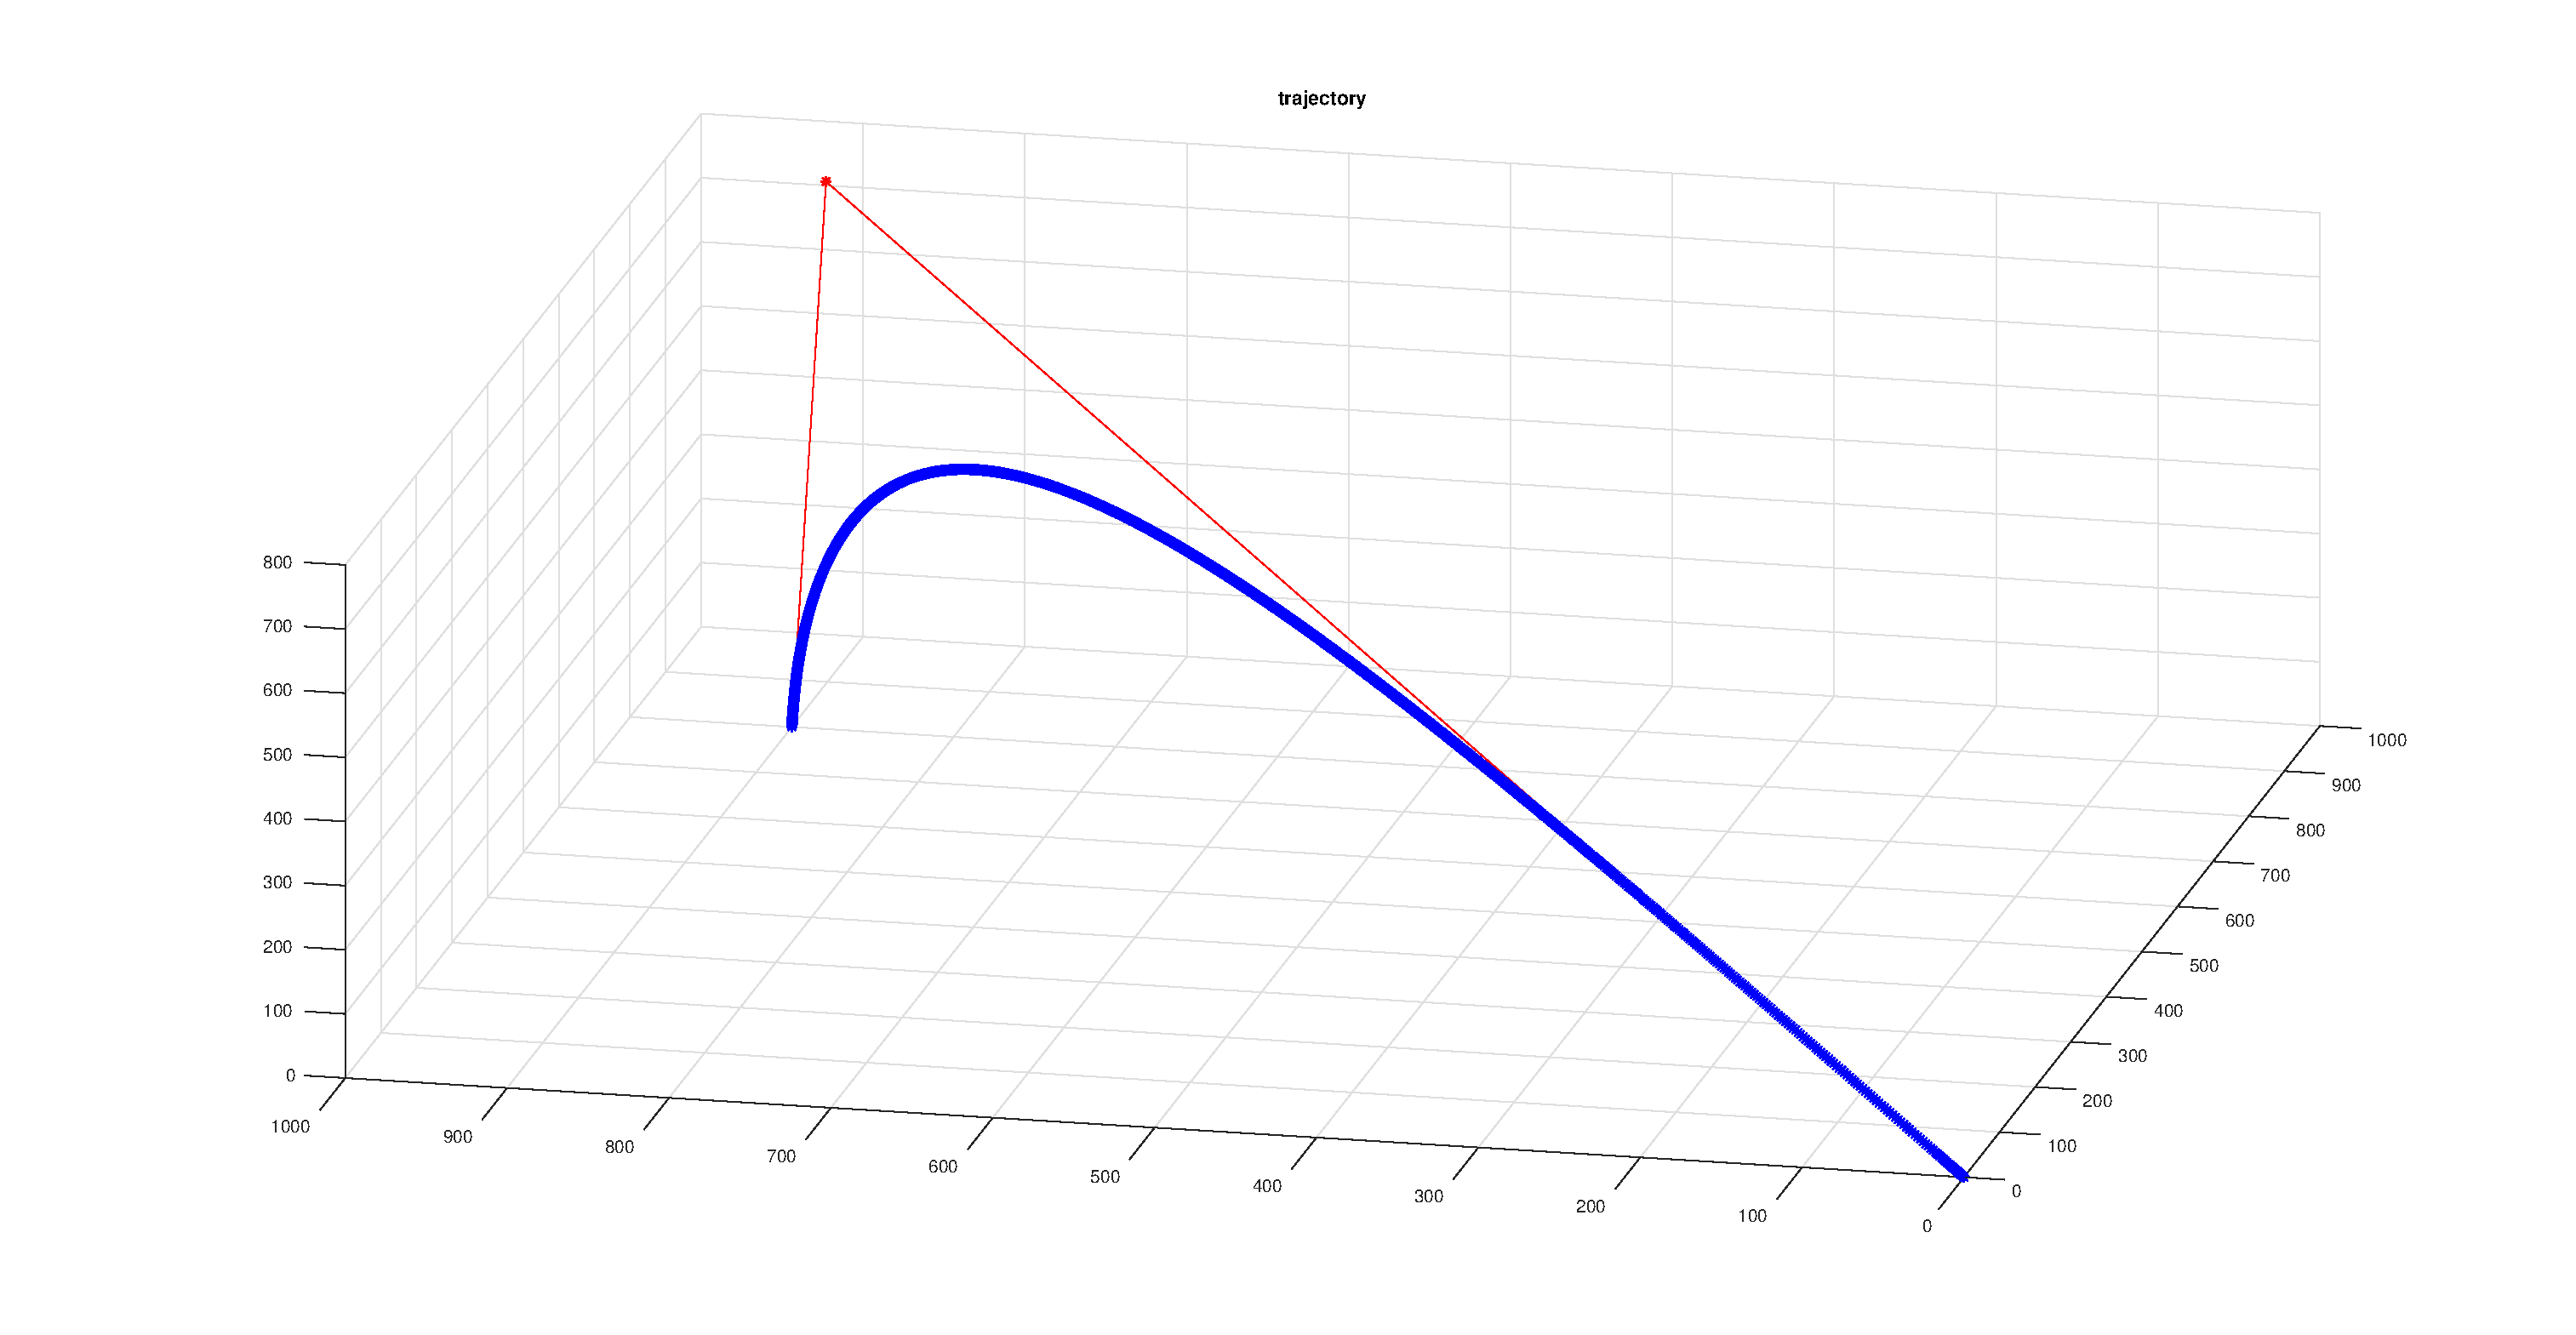
\includegraphics[height=0.6\textwidth]{motion_law_sample_problem_traj}
		\end{minipage}
		\caption[Motion Law Sample Problem]{Motion Law Sample Problem,
		left: problem layout, right: trajectory found}
		\label{fig:motion_law_sample_problem}
	\end{figure}

	\begin{figure}[hbt!]
		\centering
		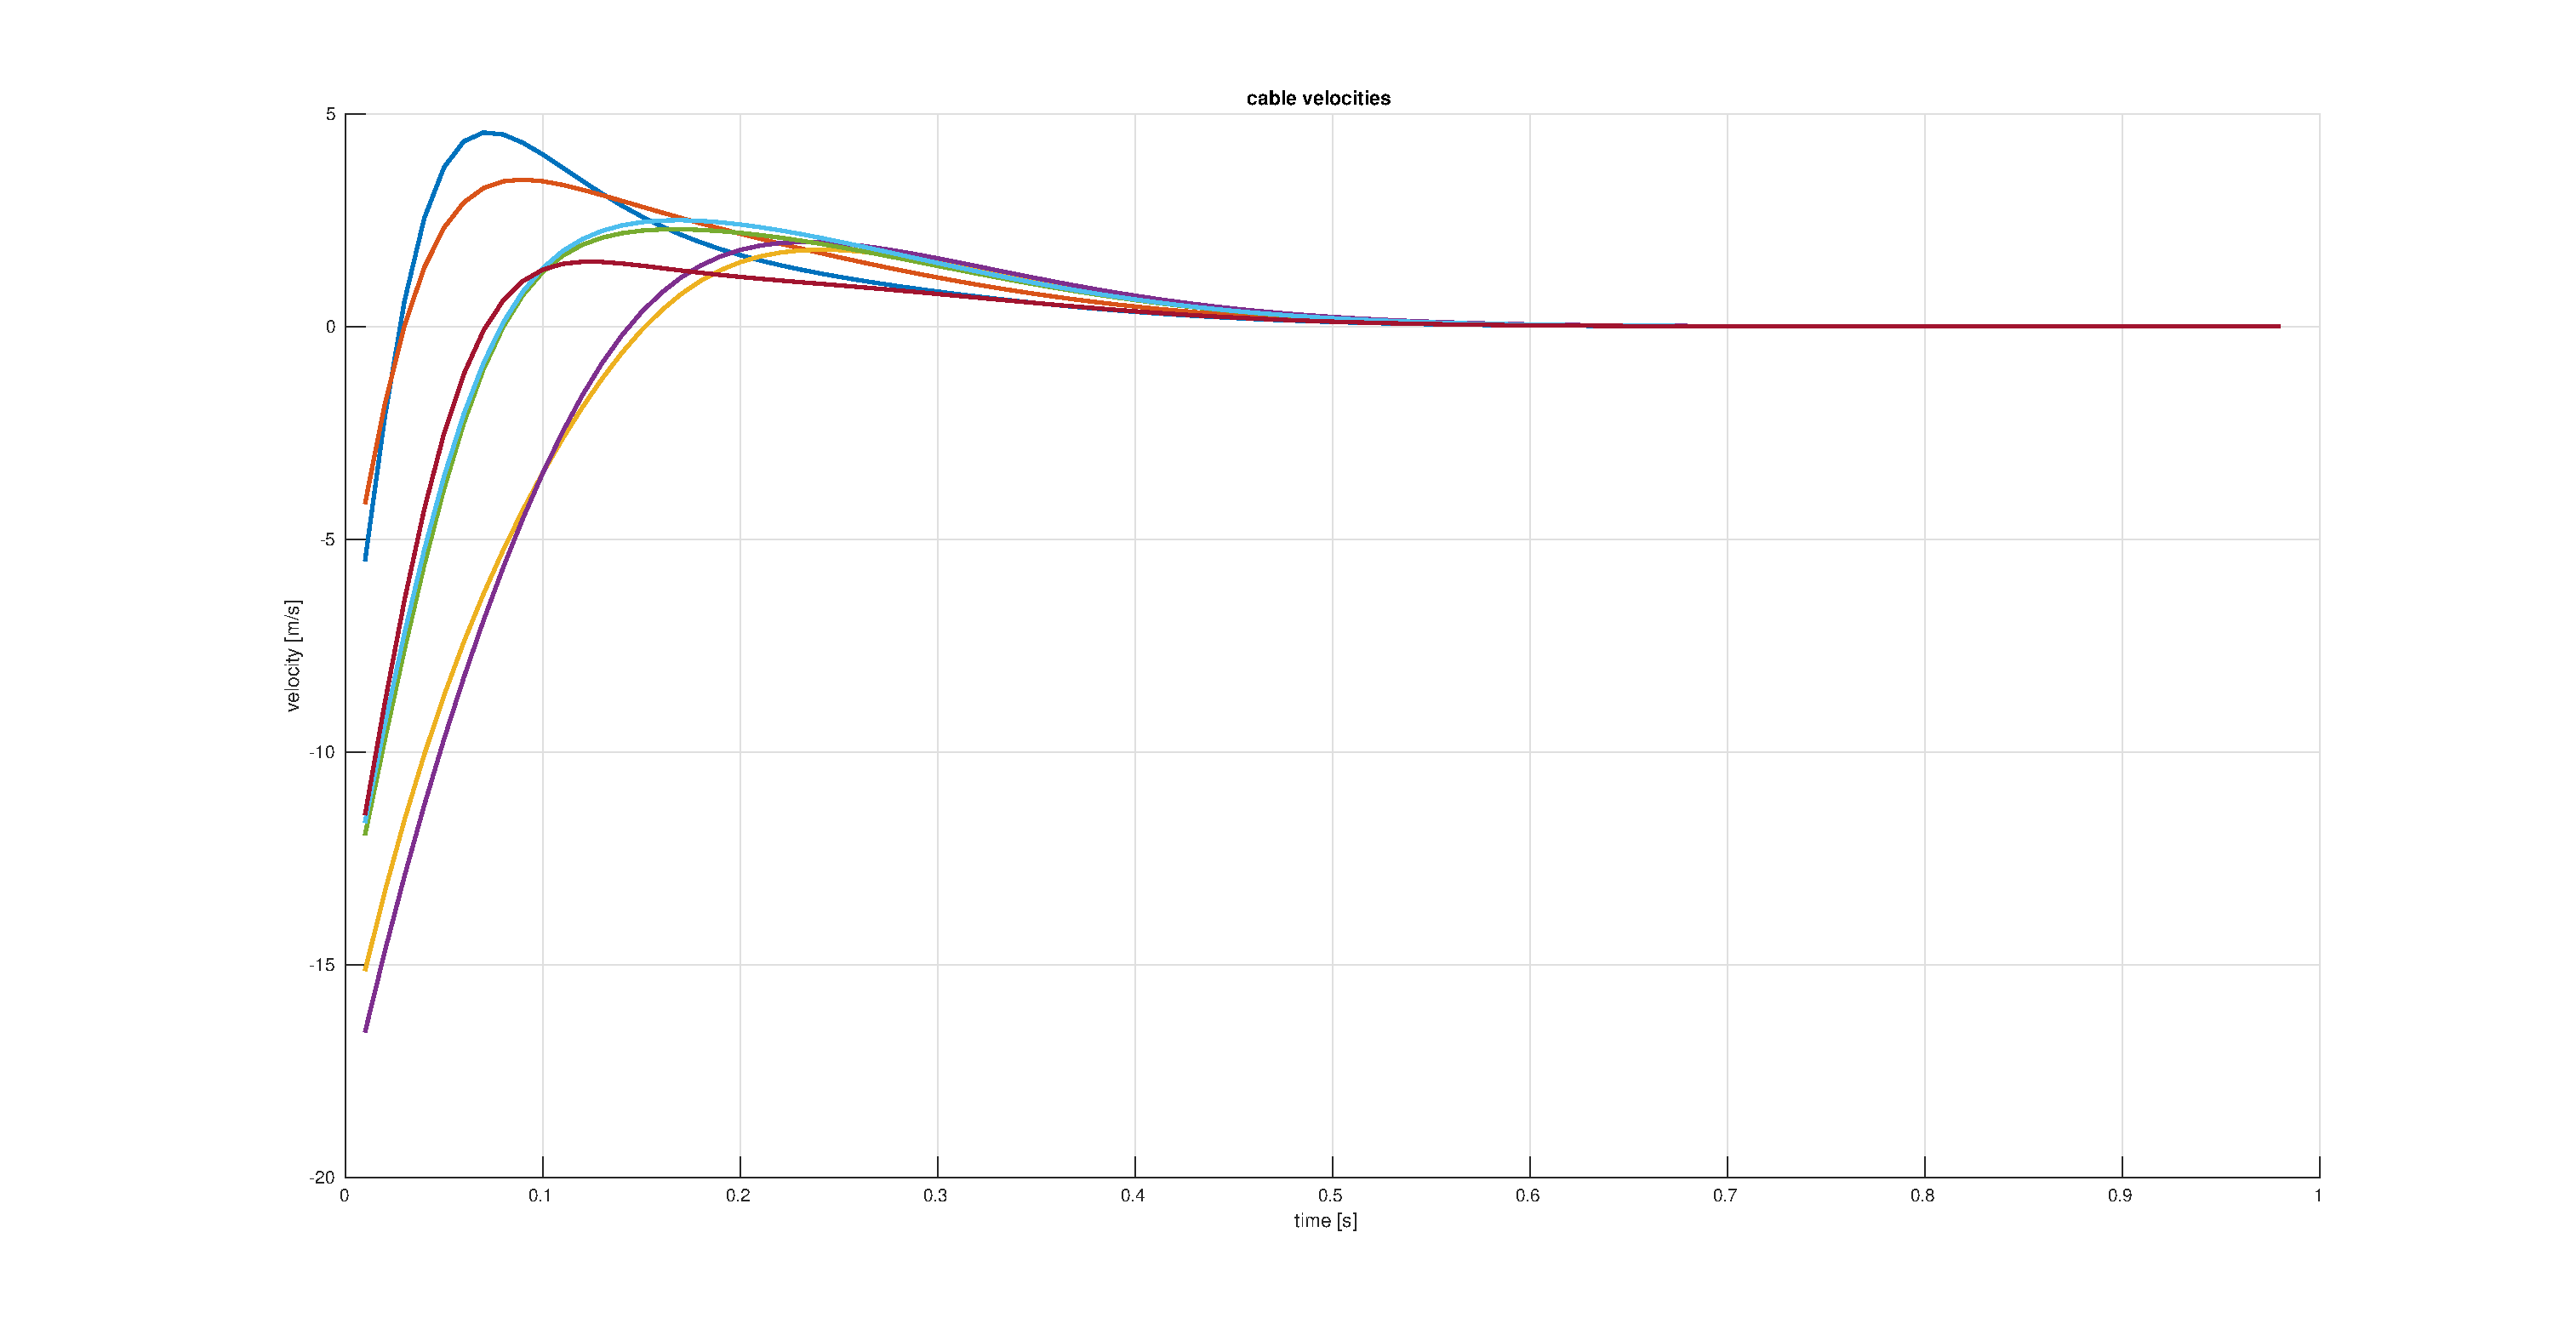
\includegraphics[width=\textwidth]{motion_law_base_velocities}
		\caption{Cable Velocities without Motion Law Scaling}
		\label{fig:cable_velocities_without_motion_law_scaling}
	\end{figure}

	\begin{figure}[hbt!]
		\centering
		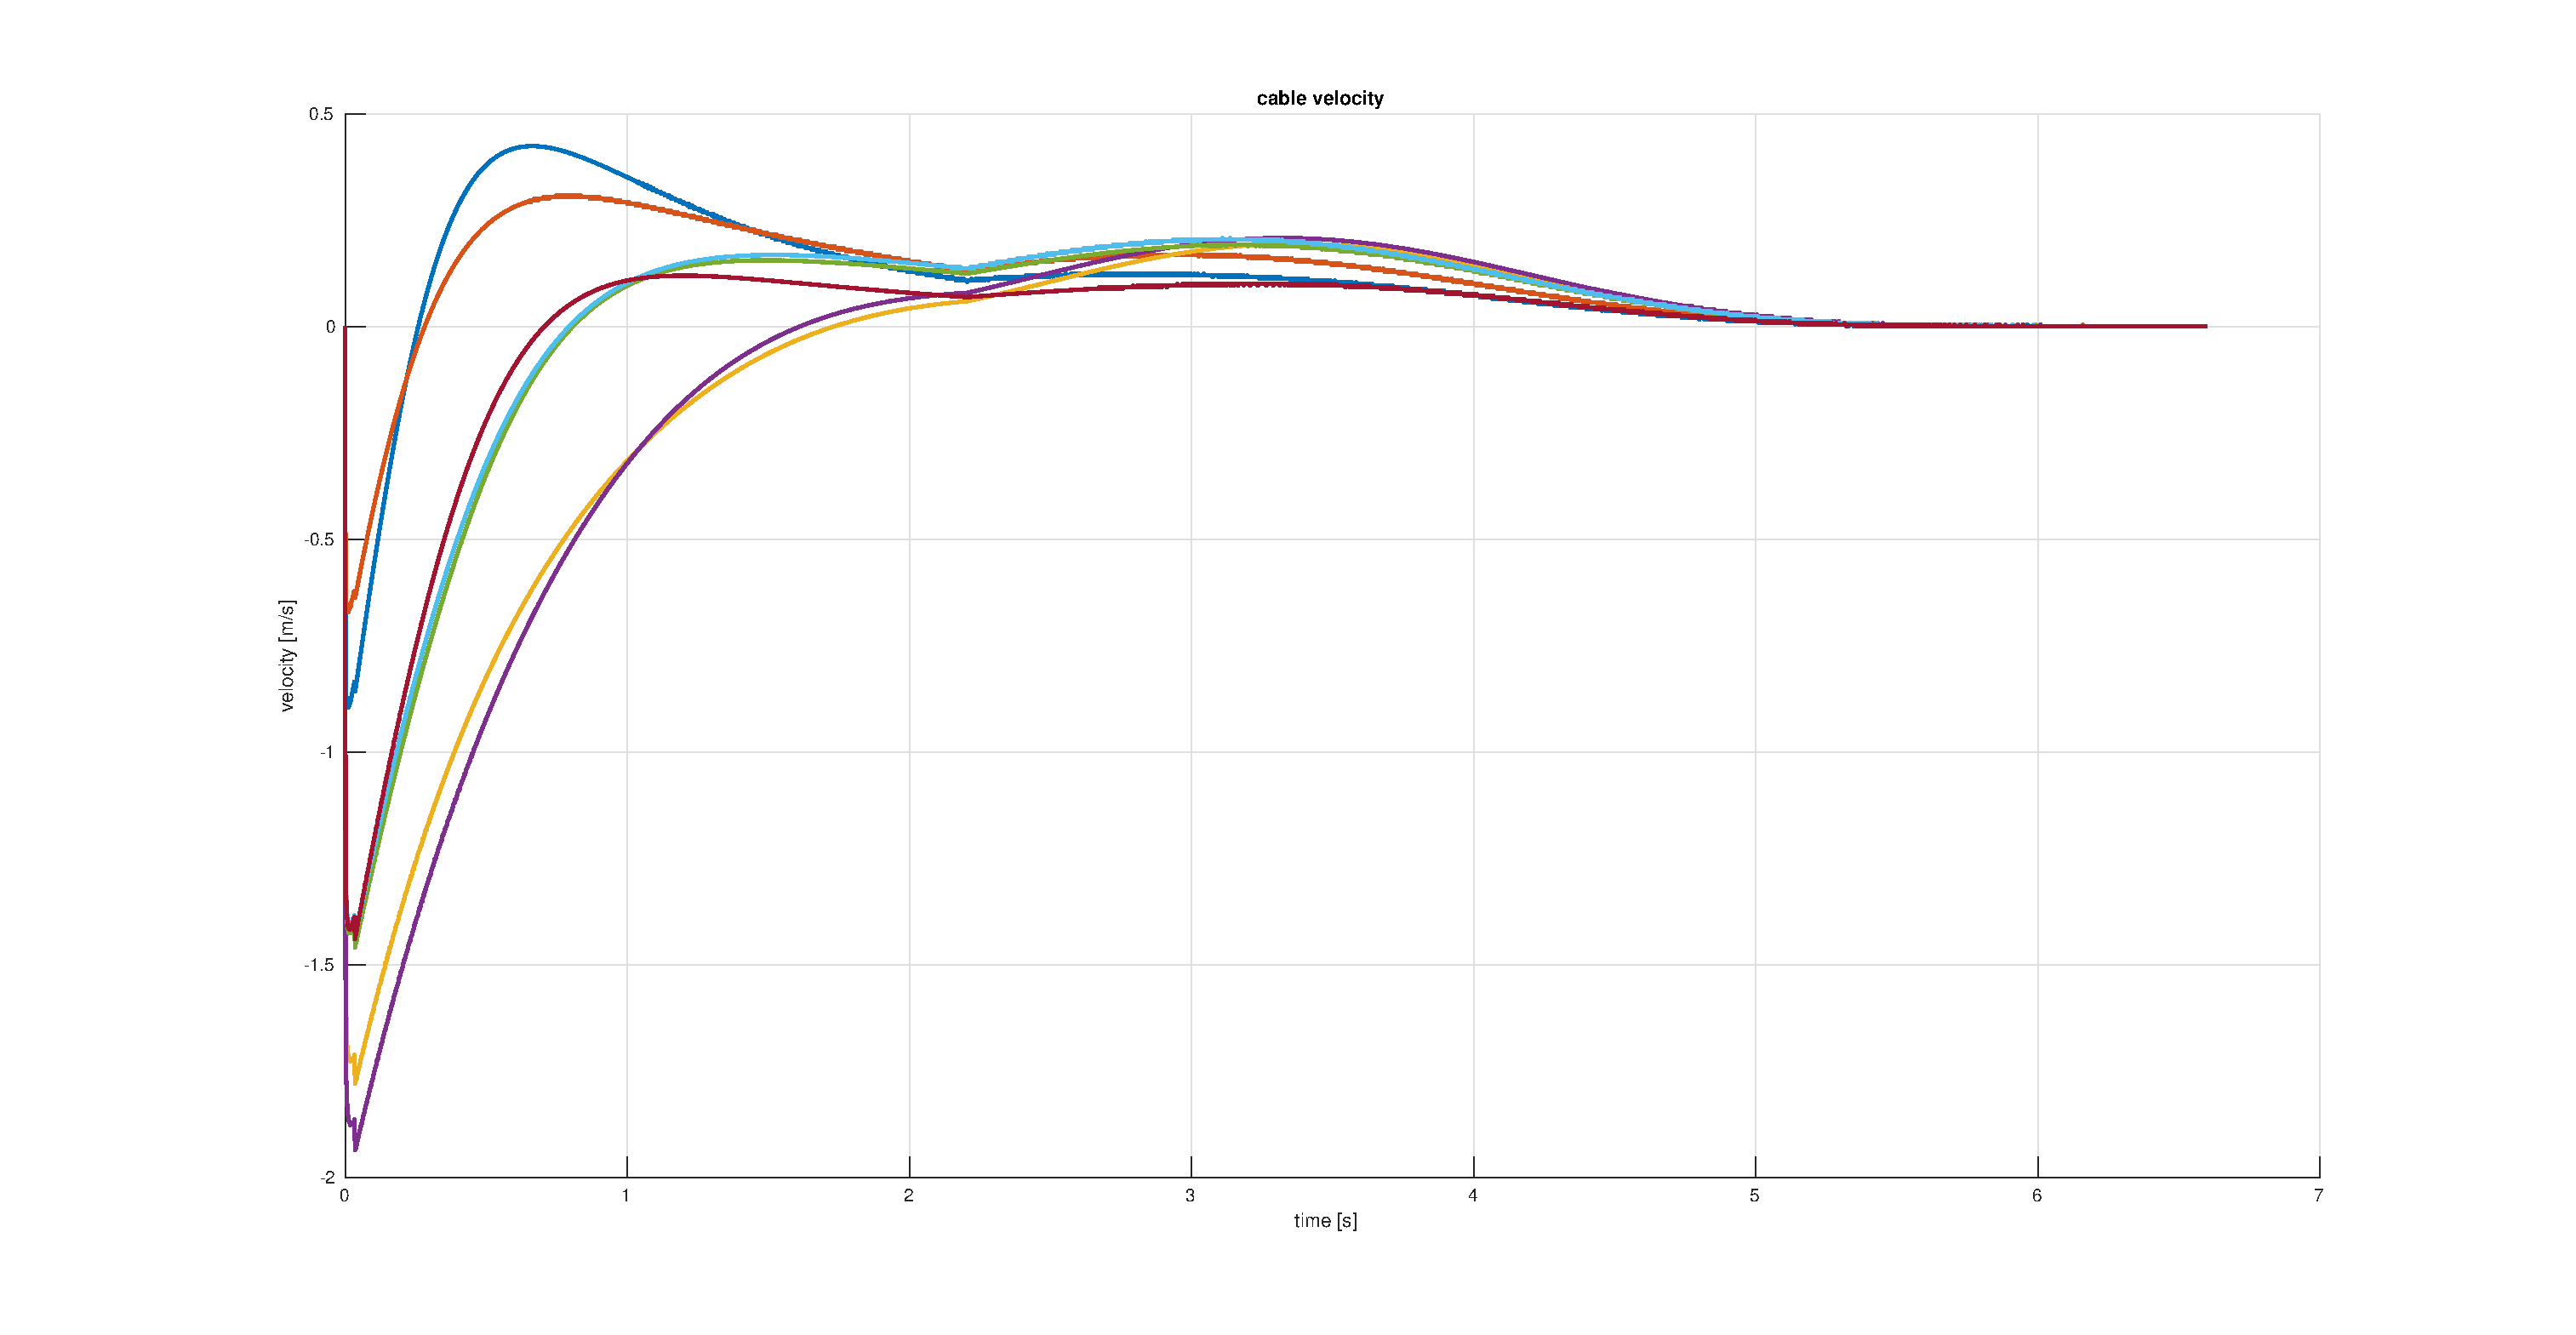
\includegraphics[width=\textwidth]{motion_law_output_velocities}
		\caption{Cable Velocities with Motion Law Scaling}
		\label{fig:cable_velocities_with_motion_law_scaling}
	\end{figure}

	\begin{figure}[hbt!]
		\centering
		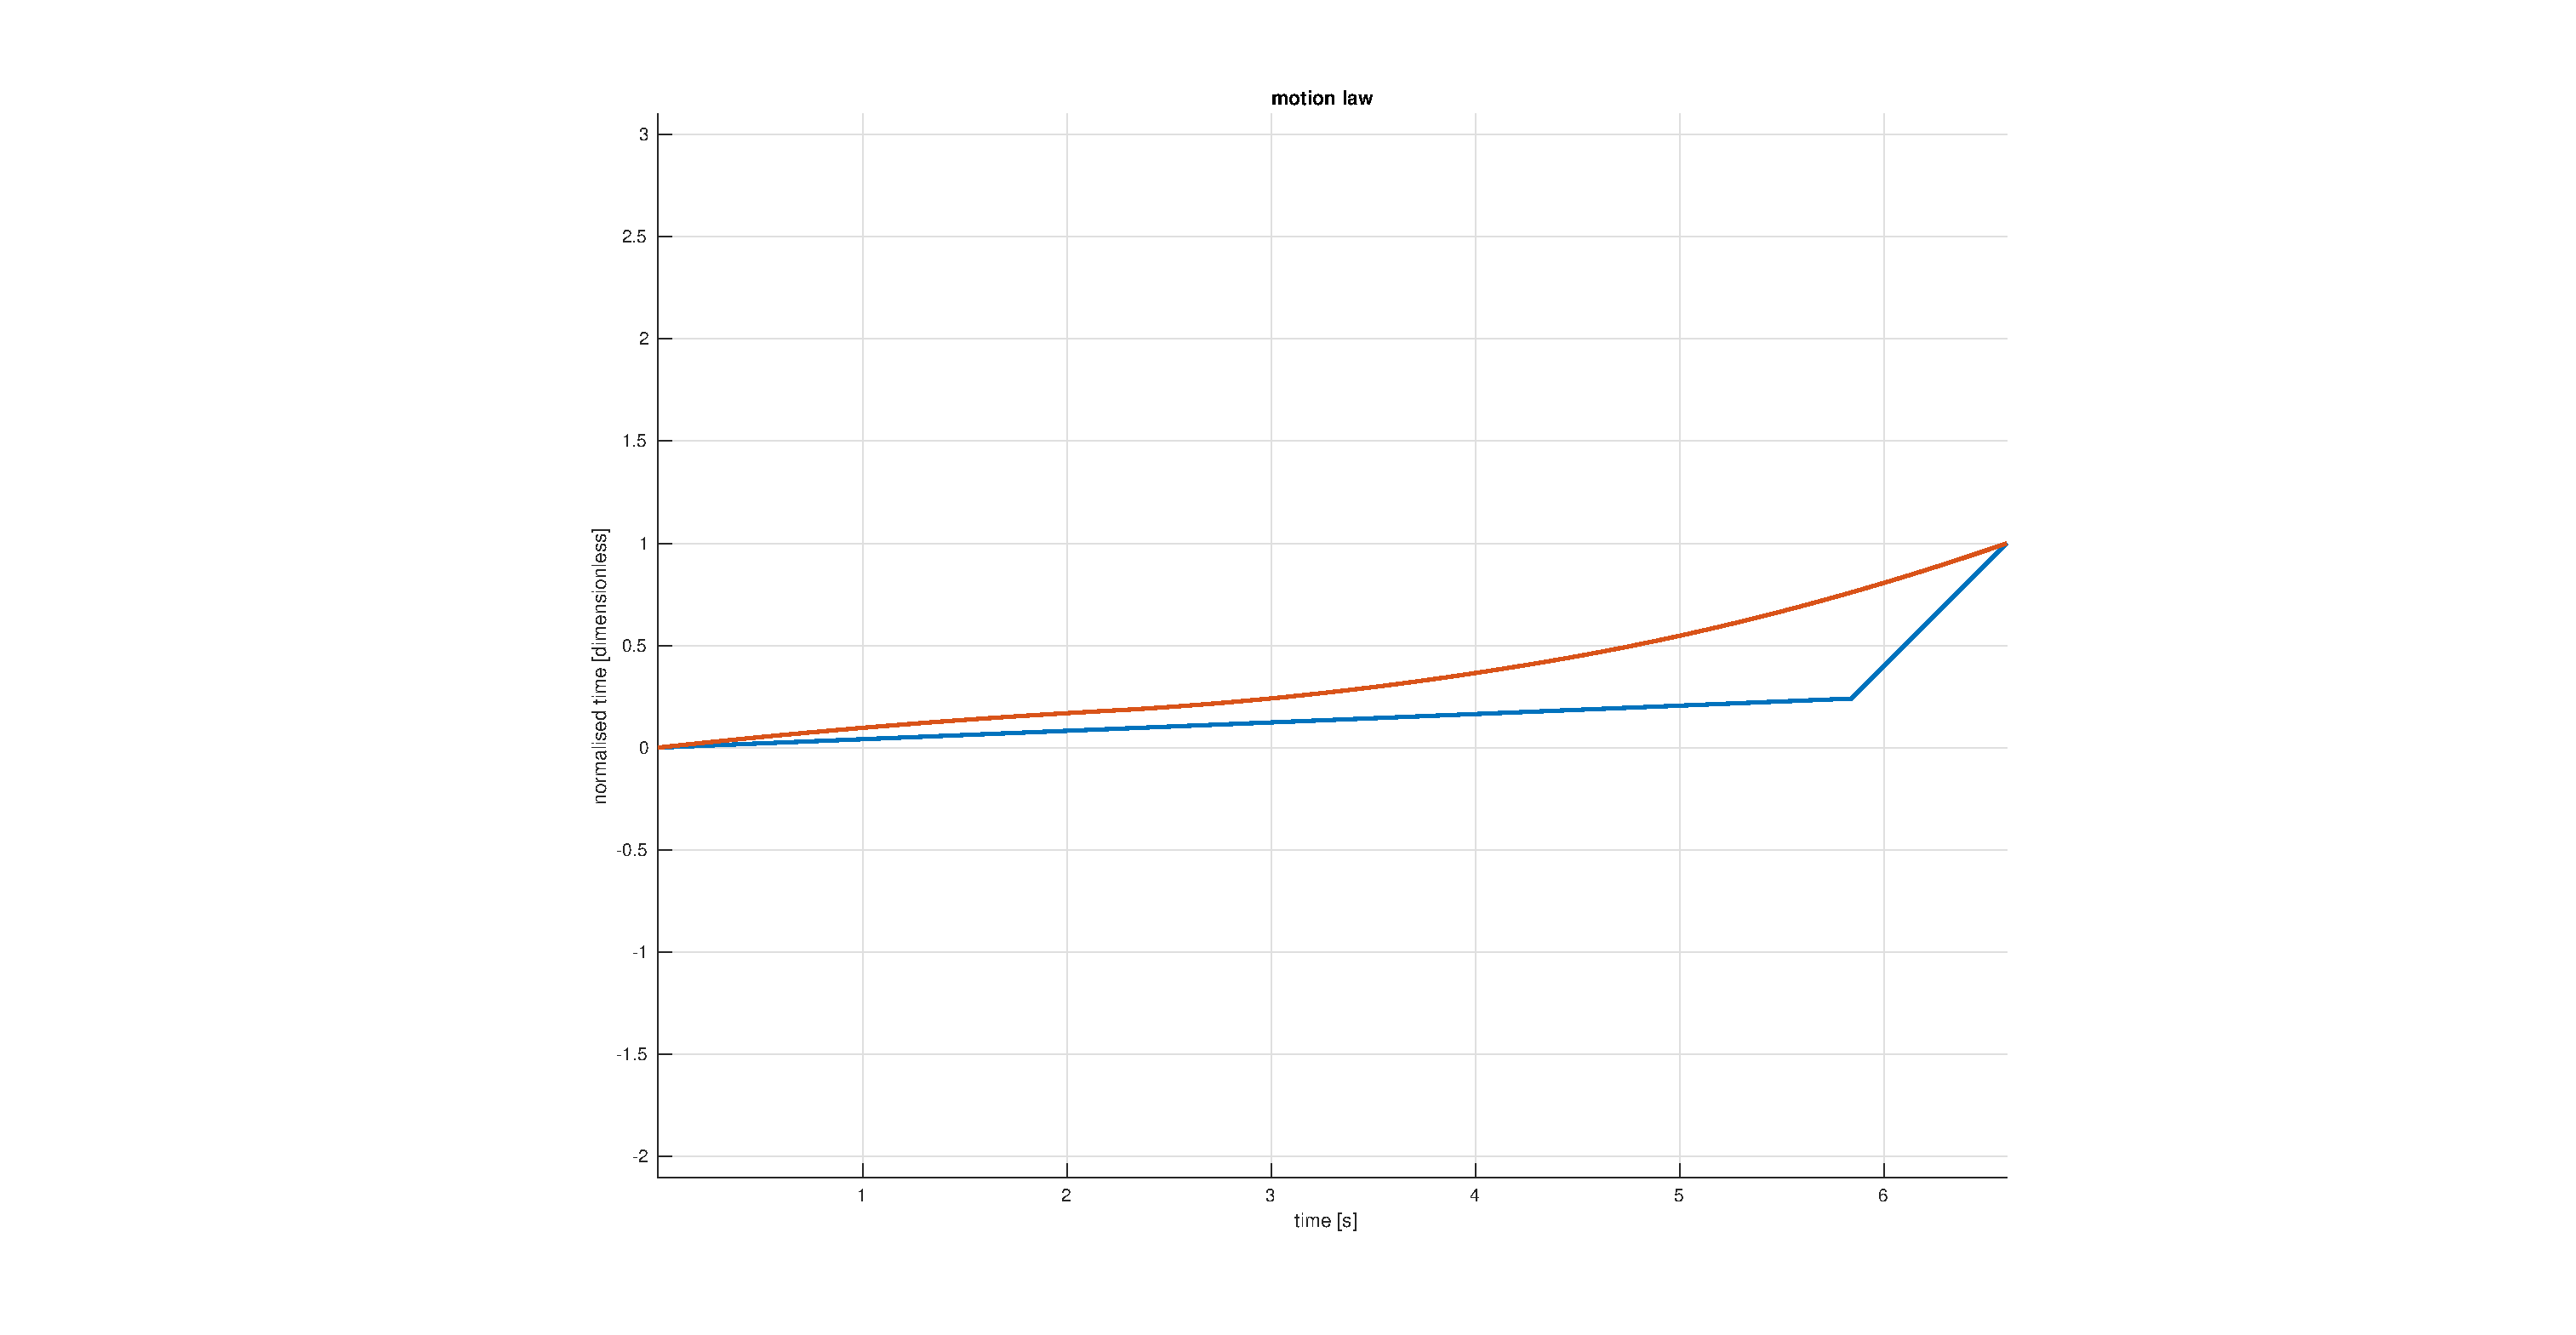
\includegraphics[width=\textwidth]{motion_law}
		\caption{Cable Velocities with Motion Law Scaling}
		\label{fig:motion_law}
	\end{figure}

	The output of the algorithm for this problem is shown in
	Figures~\ref{fig:cable_velocities_without_motion_law_scaling},
	\ref{fig:cable_velocities_with_motion_law_scaling} and~\ref{fig:motion_law}.
	In these figures, the algorithm attempted to find a motion law such that the
	maximum velocity does not exceed $2\si{\meter\per\second}$. For comparison,
	Figure~\ref{fig:cable_velocities_without_motion_law_scaling} shows the case
	where the algorithm is not applied ($\timesym \defeq \timenorm$). As can be
	seen, cable velocities reached up to $15\si{\meter\per\second}$ in this
	case. The motion law generated by the algorithm is reported in
	Figure~\ref{fig:motion_law}. In this figure both the control polygon and the
	B-Spline curve are shown. The output velocities found by applying this
	motion law is shown in
	Figure~\ref{fig:cable_velocities_with_motion_law_scaling}. As can be seen
	from the figurek the motion law succeeds in keeping the cables within their
	velocity bounds.


